\documentclass[12pt]{article}
\usepackage{xeCJK}%preamble part
\usepackage{graphicx}
\usepackage{indentfirst}
\usepackage[a4paper, inner=1.5cm, outer=3cm, top=2cm, bottom=3cm, bindingoffset=1cm]{geometry}
\usepackage{epstopdf}
\usepackage{listings}
\usepackage{array}
\usepackage{color}
\usepackage{fontspec}
\usepackage{caption}
\usepackage{subcaption}
\usepackage{bm}
\usepackage{gensymb}
\usepackage{todonotes}
\usepackage{amsmath, amsthm, amssymb}
\usepackage[citecolor=blue]{hyperref}
\newtheorem{definition}{Definition}
\newtheorem{thm}{Theorem}[section]
\newtheorem{cor}[thm]{Corollary}
\newtheorem{lem}[thm]{Lemma}
\DeclareMathOperator{\sgn}{sgn}
\theoremstyle{remark}
\newtheorem*{rem}{Remark}
\usepackage{makecell}
\setCJKmainfont[BoldFont={SimHei}]{SimSun}
\setCJKmonofont{SimSun}
\setmainfont{Times New Roman}
\newCJKfontfamily[hei]\heiti{SimHei}
\setlength{\extrarowheight}{4pt}
\setlength{\parindent}{1cm}
\definecolor{codegreen}{rgb}{0,0.6,0}
\definecolor{codegray}{rgb}{0.5,0.5,0.5}
\definecolor{codepurple}{rgb}{0.58,0,0.82}
\definecolor{backcolour}{rgb}{0.95,0.95,0.92}
\lstdefinestyle{mystyle}{
    backgroundcolor=\color{backcolour},   
    commentstyle=\color{codegreen},
    keywordstyle=\color{magenta},
    numberstyle=\tiny\color{codegray},
    stringstyle=\color{codepurple},
    basicstyle=\footnotesize,
    breakatwhitespace=false,         
    breaklines=true,                 
    captionpos=b,                    
    keepspaces=true,                 
    numbers=left,                    
    numbersep=5pt,                  
    showspaces=false,                
    showstringspaces=false,
    showtabs=false,                  
    tabsize=2
}
 
\lstset{style=mystyle}
\begin{document}
\title{\textbf{\fontsize{15.75pt}{\baselineskip}{线性常系数双曲型方程上机题目}}} 
\author{\fontsize{12pt}{\baselineskip}{数33 赵丰 \thanks{学号:2013012178} }}
\maketitle
\large
\section{题目}
考虑如下对流问题
\begin{equation}
\begin{cases}
\frac{\partial u}{\partial t}+\frac{\partial u}{\partial x}&=0\\
u(x,0)&=u_0(x),
\end{cases}
\end{equation}
分别取以下两种初值:
\begin{equation}
u_0(x)=\begin{cases}
1-\cos2\pi x,&x \in [0,1],\\
0&x \notin [0,1]
\end{cases}
\end{equation}
和

\begin{equation}
u_0(x)=\begin{cases}
1,&x \in [0.4,0.6],\\
0&x \notin [0.4,0.6]
\end{cases}
\end{equation}
进行计算,算到$T=1$,对于适中的网格比,初值取$x \in [0,2]$进行计算。计算$x_i$时使用如下的积分平均公式:
\begin{equation}
x_i=\frac{1}{h}\int_{x_{i-\frac{1}{2}}}^{x_{i+\frac{1}{2}}}u_0(x)dx
\end{equation}
\section{解析解}
\begin{equation}
u(t,x)=u_0(x-t)
\end{equation}
\section{使用的差分格式}
\subsection{迎风格式}
\begin{equation}
\frac{u_j^{n+1}-u_j^n}{\tau}+\frac{u_j^n-u_{j-1}^n}{h}=0
\end{equation}
\subsection{Lax-Friedrichs 格式}
\begin{equation}
\frac{u_j^{n+1}-\frac{1}{2}(u_{j+1}^n+u_{j-1}^n)}{\tau}+\frac{u_{j+1}^n-u_{j-1}^n}{2h}=0
\end{equation}
\subsection{Lax-Wendroff 格式}
\begin{equation}
u_j^{n+1}=u_j^n-\frac{a\lambda}{2}(u^n_{j+1}-u^n_{j-1})+\frac{a^2\lambda^2}{2}(u^n_{j+1}-2u^n_j+u^n_{j-1})
\end{equation}

其中$\lambda=\frac{\tau}{h}$为网格比

\subsection{Beam-Warming 格式}
\begin{equation}
u_j^{n+1}=u_j^n-\frac{a\lambda}{2}(3u^n_{j}-4u^n_{j-1}+u^n_{j-2})+\frac{a^2\lambda^2}{2}(u^n_{j}-2u^n_{j-1}+u^n_{j-2})
\end{equation}
\subsection{不同差分格式理论性能比较}
\section{数值结果}
用如上列出的数值格式分别求解给定的双曲问题,matlab代码如下:
\lstinputlisting[language=Matlab]{hyperbolic.m}
\section{结果分析}
\subsection{光滑初值情形}
取$h=0.01,\tau=0.011$发现结果完全不对。解释为$\lambda=\frac{\tau}{h}>1$,不满足CFL条件,以下的比较基于$h=0.1\times 10^{-k},\tau=0.9\times 10^{-k}$
计算到T=1的均方误差定义为
\begin{equation}
\text{MSE}=\sum_{j=2}^N |u_j-u_{j-1}|^2
\end{equation}
\begin{table}[!ht]
\caption{四种数值格式均方误差比较}
\centering
\begin{tabular}{|c|c|c|c|c|}
\hline
h&upwind&lax\_friedrich&lax\_wandroff&beam\_warming\\
\hline
0.01&0.038&0.099&0.0171&0.0151\\
\hline
0.001&0.022&0.028&0.0198&0.0197\\
\hline
1e-4&0.002&0.003&0.002&0.002\\
\hline
\end{tabular}
\end{table}

由上表可见,二阶格式在步长较大时精度明显高于一阶格式,但当步长逐渐缩小时,二阶格式和一阶格式的差别也在缩小。

代码在求解过程中也计算了每一步的TVD的值,对$h=0.01$的情形作图得:

\begin{figure}[!ht]
\centering
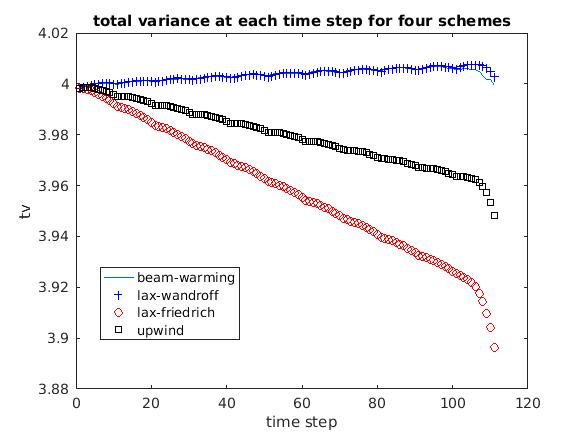
\includegraphics[width=400pt]{tvd.jpg}
\end{figure}

通过上图可以看出,两个一阶的格式确实是TVD的格式,而两个二阶的格式随时间步长的增大全变差增大,因此不是TVD的格式。
\subsection{非光滑初值情形}
求解由(2)给出的初值时,由于初值不连续,无论用什么格式T=1时的解误差均比较大,一阶格式给出的解是将初值的不连续性磨光,如下面左图所示;二阶格式给出的解在初值不连续点出现振荡的现象,如下面的右图所示。
\begin{figure}[!ht]
\centering
\begin{subfigure}{0.4\textwidth}
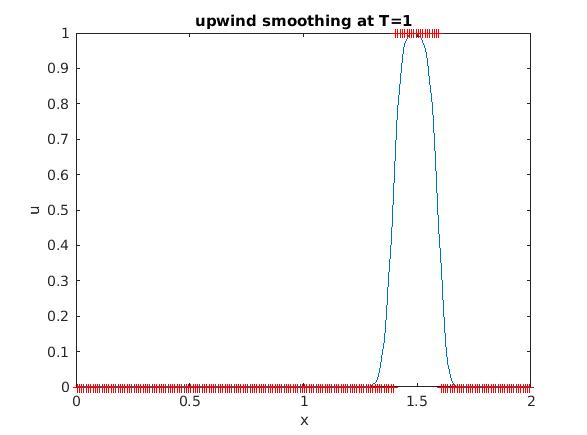
\includegraphics[width=\textwidth]{smoothing.jpg}
\end{subfigure}
\begin{subfigure}{0.4\textwidth}
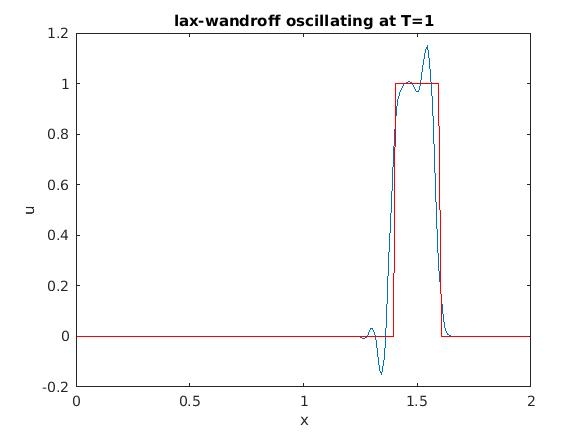
\includegraphics[width=\textwidth]{oscillating.jpg}
\end{subfigure}
\end{figure}

\section{结论}
通过这次上机实验熟悉了使用显式两层差分格式求解双曲问题的思路。
\end{document}
